\section{Results}

Current results include typical time histories for quantities of interest. Namely steam demand, electric demand, and power produced by VRE. Thus the first step of the methodology from Baker et. al has been completed.

\begin{figure}[H]
 	\centering
 	\label{grid-demand}
 	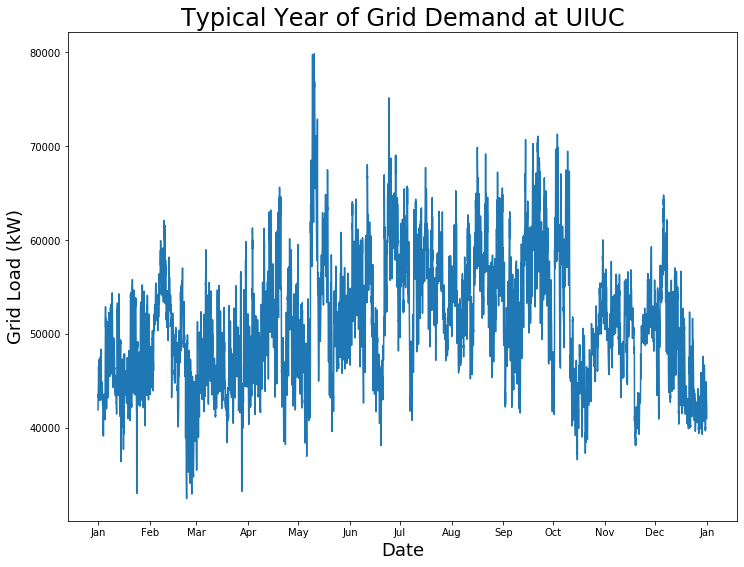
\includegraphics[width=0.8\columnwidth]{typical_grid_demand.png}
 	\caption{The typical year of hourly grid demand in kW at UIUC.}
\end{figure} 
\begin{figure}[H]
	\centering
	\label{steam-demand}
	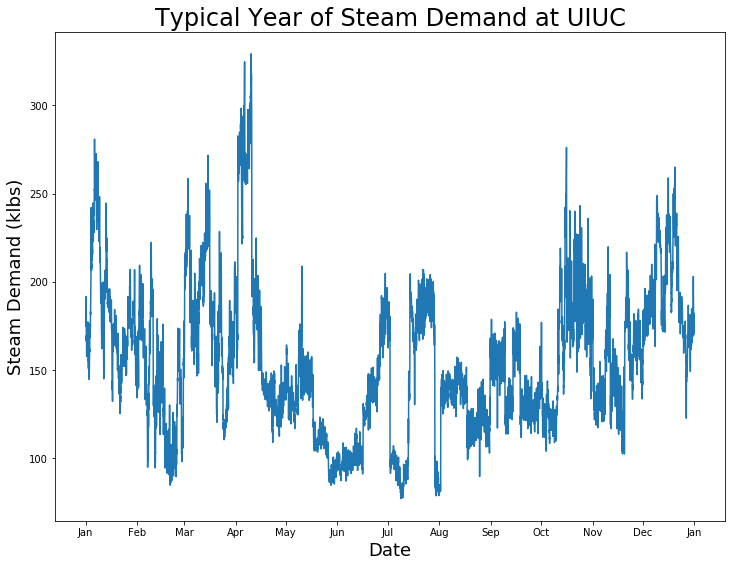
\includegraphics[width=0.8\columnwidth]{typical_steam_demand.png}
	\caption{The typical year of hourly steam demand in kW at UIUC.}
\end{figure}
\begin{figure}[H]
	\centering
	\label{solar-power}
	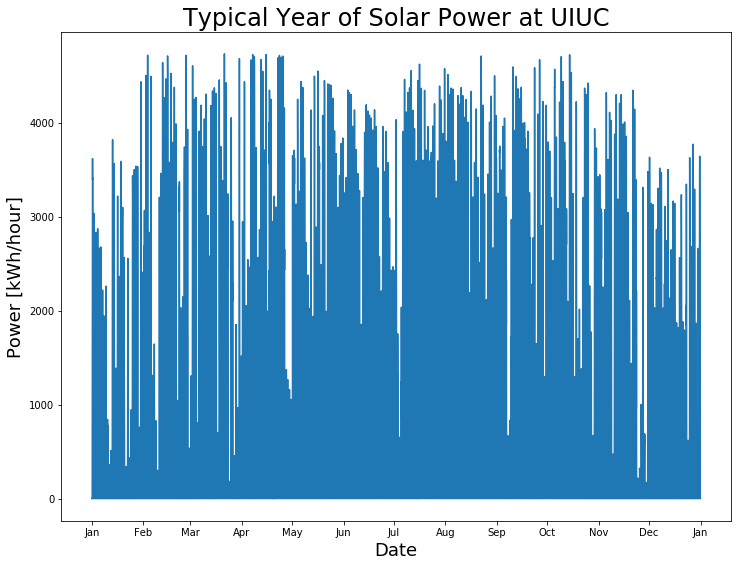
\includegraphics[width=0.8\columnwidth]{typical_solar_power.png}
	\caption{The typical year of hourly power produced by the UIUC solar farm.}
\end{figure}
\begin{figure}[H]
	\centering
	\label{wind-power}
	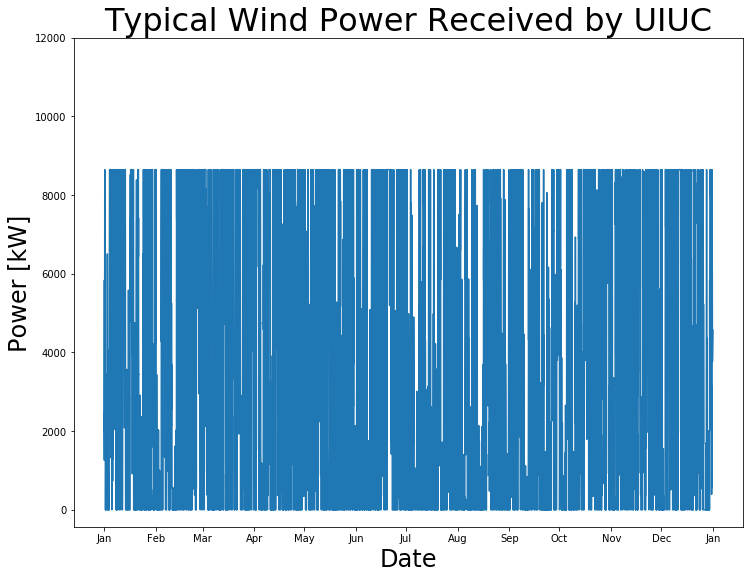
\includegraphics[width=0.8\columnwidth]{typical_wind_v3.png}
	\caption{The typical year of hourly wind power received by UIUC.}
\end{figure}